\documentclass[aspectratio=169]{beamer}
\usepackage{will_handley_beamer}
\usepackage{title_page}
\usetikzlibrary{positioning, calc, arrows.meta, shapes}

% Commands
% --------
% - \arxiv{arxiv number}
% - \arxiv{<number>}            arxiv.org/abs/<number>
% - \oldarxiv{<arxiv number>}   arxiv.org/<number>
% - \doi{<doi>}                 doi.org/<doi>
% - \xkcd{<number>}             xkcd.com/<number>
% - \email{<email>}             <<email>>
% - \tthref{<website>}          <website>
% - \av[dist]{<quantity>}       <quantity>_{dist}
% - \student{<name>}{<detail>}{<photo>}

% Talk details
% ------------
\title{Theory meets experiment 2025}
\subtitle{New frontiers in particle cosmology}
\date{7\textsuperscript{th} January 2024}

\begin{document}

\begin{frame}
    \titlepage
\end{frame}

\begin{frame}
    \frametitle{TMEX: Theory meets experiment}
    \framesubtitle{New frontiers in particle cosmology}

    \centerline{%
        \begin{tikzpicture}[
                every node/.style={align=center, font=\bfseries},
                box/.style={draw, rounded corners, minimum width=2cm, minimum height=1cm, fill=C2!30},
                trapezoid/.style={draw, trapezium, minimum width=2cm, minimum height=1cm, trapezium stretches body, fill=C1!50},
                ellipsoid/.style={draw, ellipse, minimum width=2cm, minimum height=1cm, fill=C0!50},
                cloudoid/.style={draw, cloud, cloud puffs=10, aspect=2, inner ysep=1em, fill=C3!30}, % Cloud style
                arrow/.style={thick, -{Stealth[length=3mm, width=2mm]}}
            ]

            \node[ellipsoid] (theory) {\Large Theory};
            \node[trapezoid] (experiment) at (6,0) {\Large Experiment};

            \node[box] (forward) at (3,1.5) {Forward Model};
            \node[cloudoid] (inference) at (3,-1.5) {Inference}; % Cloud shape

            \draw[arrow] (theory) to[bend left=25]  (forward);
            \draw[arrow] (forward) to[bend left=25] (experiment);

            \draw[arrow] (experiment) to[bend left=25] (inference);
            \draw[arrow] (inference) to[bend left=25] (theory);

        \end{tikzpicture}
    }

    \begin{columns}
        \column{0.5\textwidth}
        \begin{itemize}
            \item Inference sits at the interface between theory~and~experiment
            \item Also called ``inverse problems''
            \item Process is direct: ``measurement''
        \end{itemize}
        
        \column{0.5\textwidth}
        \begin{itemize}
            \item This talk focuses on \textbf{frontiers}:
        \end{itemize}
        \begin{enumerate}
            \item Simulation-based inference
            \item GPU-accelerated inference
        \end{enumerate}
    \end{columns}
\end{frame}

\begin{frame}
    \frametitle{Bayesian \& frequentist data combination}
    \framesubtitle{Multimessenger approaches}
    \begin{columns}
        \column{0.45\textwidth}
        \begin{block}{Frequentist}
            \begin{itemize}
                \item Preferred by particle physicists \& mathematicians
                \item Probability/stochasticity only in the data $D$
            \end{itemize}
        \end{block}
        \column{0.45\textwidth}
        \begin{block}{Bayesian}
            \begin{itemize}
                \item Preferred by astronomers \& machine learning/information theorists
                \item Quantifies all uncertainties in data \& model $(D,\theta,M)$ using probability.
            \end{itemize}
        \end{block}
    \end{columns}
    \vspace{10pt}
    \begin{columns}
        \column{0.5\textwidth}
        \begin{itemize}
            \item Whether Bayesian or frequentist, If you have a model $M$ with parameters $\theta$, multiple datasets combine at the likelihood level:
                \[ P(D_1,D_2|\theta, M) = P(D_1|\theta, M)P(D_2|\theta, M) \]
                \[ \mathcal{L}_{\text{joint}} = \mathcal{L}_1 \times \mathcal{L}_2 \times \ldots \times \mathcal{L}_n \]
        \end{itemize}
        \column{0.5\textwidth}
        \begin{overpic}[width=\textwidth]{figures/overlay}
            \put(40,0) {\tiny\arxiv{2012.09874}}
        \end{overpic}
    \end{columns}
\end{frame}

\begin{frame}
    \frametitle{An aside: difference in plotting}
    \framesubtitle{Exclusion vs.\  posterior plots}
    %examples of bad practice, e.g. PTA data
\end{frame}

\begin{frame}
    \frametitle{The three pillars of (Bayesian) inference}
    \begin{columns}[t]
        \column{0.33\textwidth}
        \begin{block}{Parameter estimation}
            What do the data tell us about the parameters of a model?\\
            {\textit{e.g. the size or age of a $\Lambda$CDM universe}}%
            \[ \hspace{-4pt}\C[0]{P(\theta|D,M)} = \frac{\C[2]{P(D|\theta,M)} \C[1]{P(\theta|M)}}{\C[3]{P(D|M)}} \] 
            \[ \C[0]{\mathcal{P}} = \frac{\C[2]{\mathcal{L}} \times\C[1]{\pi}}{\C[3]{\mathcal{Z}}}\] 
            \[ \C[0]{\text{Posterior}} = \frac{\C[2]{\text{Likelihood}} \times\C[1]{\text{Prior}}}{\C[3]{\text{Evidence}}}\]
        \end{block}
        \column{0.3\textwidth}
        \begin{block}{Model comparison}
            How much does the data support a particular model?\\
            {\textit{e.g. $\Lambda$CDM vs a dynamic dark energy cosmology}}%
            \[ \C[5]{P(M|D)} = \frac{\C[3]{P(D|M)} \C[6]{P(M)}}{\C[7]{P(D)}} \vspace{-7pt}\]
            \[ \frac{\C[3]{\mathcal{Z}_{M}} \C[6]{\Pi_{M}}}{\C[7]{\sum_m Z_m \Pi_m}} \]
            \[ \C[5]{\text{Posterior}} = \frac{\C[3]{\text{Evidence}} \times\C[6]{\text{Prior}}}{\C[7]{\text{Normalisation}}}\]
        \end{block}
        \column{0.33\textwidth}
        \begin{block}{Tension quantification}
            Do different datasets make consistent predictions from the same model? 
            {\textit{\textit{e.g. CMB vs Type IA supernovae data}}}%
            \[ \mathcal{R} = \frac{\C[3]{\mathcal{Z}}_{AB}}{\C[3]{\mathcal{Z}}_A\C[3]{\mathcal{Z}}_\mathcal{B}}\] 
            \[
                \begin{aligned} \log\mathcal{S} = \av[{\C[0]{\mathcal{P}}_{AB}}]{\C[2]{\log\mathcal{L}}_{AB}}&\\
                    -\av[{\C[0]{\mathcal{P}}_{A}}]{\C[2]{\log\mathcal{L}}_{A}}&\\
                    -\av[{\C[0]{\mathcal{P}}_{B}}]{\C[2]{\log\mathcal{L}}_{B}}&
                \end{aligned}
            \]
        \end{block}
    \end{columns}
\end{frame}

\section{Likelihood-based inference}
\begin{frame}
    \frametitle{LBI: Likelihood-based inference}
    \begin{columns}
        \column{0.5\textwidth}
        The standard approach if you are fortunate enough to have a likelihood function $\only<1-2>{P(D|\theta)}\only<3->{\C[2]{\mathcal{L}(D|\theta)}}$: 
        \[
            \only<1-2>{
                P(\theta|D) = \frac{P(D|\theta)P(\theta)}{P(D)}
            }
            \only<2>{
                \qquad
                \C[0]{\text{Posterior}} = \frac{\C[2]{\text{Likelihood}}\times\C[1]{\text{Prior}}}{\C[3]{\text{Evidence}}}
            }
            \only<3>{
                \C[0]{\mathcal{P}(\theta|D)} = \frac{\C[2]{\mathcal{L}(D|\theta)}\C[1]{\pi(\theta)}}{\C[3]{\mathcal{Z}(D)}}
                \qquad
                \C[0]{\text{Posterior}} = \frac{\C[2]{\text{Likelihood}}\times\C[1]{\text{Prior}}}{\C[3]{\text{Evidence}}}
            }
            \only<4>{
                \C[0]{P(\theta|D)} \C[3]{P(D)} = \C[4]{P(\theta,D)} = \C[2]{P(D|\theta)}\C[1]{P(\theta)}, \qquad
            }
            \only<5>{
                \C[0]{\mathcal{P}}\times\C[3]{\mathcal{Z}} = \C[4]{\mathcal{J}} = \C[2]{\mathcal{L}}\times\C[1]{\pi}, \qquad \C[4]{\text{Joint}} = \C[4]{\mathcal{J}} = P(\theta,D)
            }
        \]
        \vspace{-10pt}
        \begin{enumerate}
            \item Define \C[1]{prior $\pi(\theta)$} 
                \begin{itemize}
                    \item spend some time being philosophical
                \end{itemize}
            \item Sample \C[0]{posterior $\mathcal{P}(\theta|D)$} 
                \begin{itemize}
                    \item use out-of-the-box MCMC tools such as\\ \texttt{emcee} or \texttt{MultiNest}
                    \item make some triangle plots
                \end{itemize}
            \item Optionally compute \C[3]{evidence $\mathcal{Z}(D)$}
                \begin{itemize}
                    \item e.g. nested sampling or parallel tempering
                    \item do some model comparison (i.e. science)
                    \item talk about tensions
                \end{itemize}
        \end{enumerate}
        \column{0.5\textwidth}
        \hfill%
        \begin{overpic}[width=0.6\textwidth]{figures/des_parameters.pdf}
            \put(-40,90) {DES Y5 SN Ia}
            \put(-40,80) {\arxiv{2401.02929}}
        \end{overpic}
        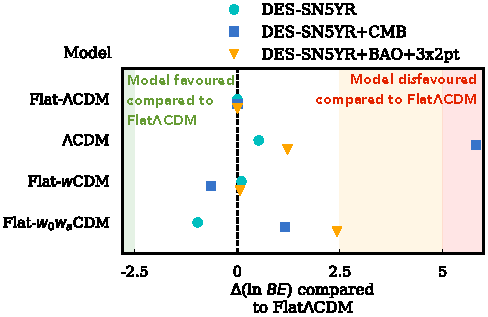
\includegraphics[width=0.5\textwidth]{figures/des_model_comparison.pdf}%
        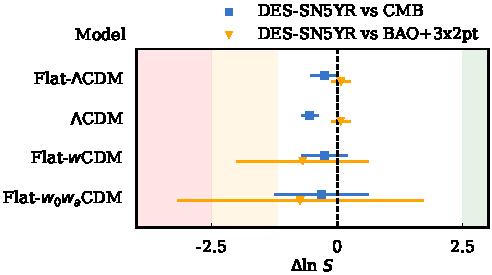
\includegraphics[width=0.5\textwidth]{figures/des_suspiciousness.pdf}
    \end{columns}
\end{frame}


\section{Simulation-based inference}
\subsection{Principles \& motivation}
\begin{frame}
    \frametitle{SBI: Simulation-based inference}
    \begin{columns}
        \column{0.5\textwidth}
        \begin{itemize}
            \item What do you do if you don't know \C[2]{$\mathcal{L}(D|\theta)$}?
            \item If you have a simulator/forward model $\theta \rightarrow D$
                defines an \C[2]{\emph{implicit} likelihood~$\mathcal{L}$}.
            \item Simulator generates samples from $\C[2]{\mathcal{L}(\cdot|\theta)}$.
            \item With a prior $\C[1]{\pi}(\theta)$ can generate samples from \C[4]{joint distribution}~$\C[4]{\mathcal{J}(\theta,D)}=\C[2]{\mathcal{L}(D|\theta)}\C[1]{\pi(\theta)}$\\\hfill \emph{the ``probability of everything''}.
            \item Task of SBI is take joint~$\C[4]{\mathcal{J}}$ samples and learn \C[0]{posterior $\mathcal{P}(\theta|D)$} and \C[3]{evidence $\mathcal{Z}(D)$} \\\hfill and possibly \C[2]{likelihood $\mathcal{L}(D|\theta)$}.
            \item Present state of the art achieves this using \emph{machine learning} (neural networks).
                \begin{itemize}
                    \item My group's research tries to removes machine learning \tthref{github.com/handley-lab/lsbi}.
                \end{itemize}
        \end{itemize}
        \column{0.5\textwidth}
        \includegraphics<1>[page=1, width=\textwidth]{figures/sbi_parameter_estimation.pdf}%
        \includegraphics<2>[page=2, width=\textwidth]{figures/sbi_parameter_estimation.pdf}%
        \includegraphics<3>[page=3, width=\textwidth]{figures/sbi_parameter_estimation.pdf}%
        \includegraphics<4>[page=4, width=\textwidth]{figures/sbi_parameter_estimation.pdf}%
        \includegraphics<5>[page=5, width=\textwidth]{figures/sbi_parameter_estimation.pdf}%
        \includegraphics<6>[page=6, width=\textwidth]{figures/sbi_parameter_estimation.pdf}%
        \includegraphics<7>[page=7, width=\textwidth]{figures/sbi_parameter_estimation.pdf}%
        \includegraphics<8>[page=8, width=\textwidth]{figures/sbi_parameter_estimation.pdf}%
        \includegraphics<9>[page=9, width=\textwidth]{figures/sbi_parameter_estimation.pdf}%
        \includegraphics<10>[page=10, width=\textwidth]{figures/sbi_parameter_estimation.pdf}%
        \includegraphics<11>[page=11, width=\textwidth]{figures/sbi_parameter_estimation.pdf}%
        \includegraphics<12>[page=12, width=\textwidth]{figures/sbi_parameter_estimation.pdf}%
        \includegraphics<13>[page=13, width=\textwidth]{figures/sbi_parameter_estimation.pdf}%
        \includegraphics<14>[page=14, width=\textwidth]{figures/sbi_parameter_estimation.pdf}%
        \includegraphics<15>[page=15, width=\textwidth]{figures/sbi_parameter_estimation.pdf}%
        \includegraphics<16>[page=16, width=\textwidth]{figures/sbi_parameter_estimation.pdf}%
        \includegraphics<17>[page=17, width=\textwidth]{figures/sbi_parameter_estimation.pdf}%
        \includegraphics<18>[page=18, width=\textwidth]{figures/sbi_parameter_estimation.pdf}%
        \includegraphics<19>[page=19, width=\textwidth]{figures/sbi_parameter_estimation.pdf}%
        \includegraphics<20>[page=20, width=\textwidth]{figures/sbi_parameter_estimation.pdf}%
        \includegraphics<21>[page=21, width=\textwidth]{figures/sbi_parameter_estimation.pdf}%
    \end{columns}
\end{frame}

\begin{frame}
    \frametitle{Why SBI?}
    \begin{columns}
        \column{0.6\textwidth}
        SBI is useful because:
        \begin{enumerate}
            \item If you don't have a likelihood, you can still do inference
                \begin{itemize}
                    \item This is the usual case beyond CMB cosmology
                \end{itemize}
            \item Faster than LBI
                \begin{itemize}
                    \item emulation -- also applies to LBI in principle
                \end{itemize}
            \item No need to pragmatically encode fiducial cosmologies
                \begin{itemize}
                    \item Covariance computation implicitly encoded in simulations
                    \item Highly relevant for disentangling tensions \& systematics
                \end{itemize}
            \item Equips AI/ML with Bayesian interpretability
            \item Lower barrier to entry than LBI
                \begin{itemize}
                    \item Much easier to forward model a systematic
                    \item Emerging set of plug-and-play packages
                    \item For this reason alone, it will come to dominate scientific inference
                \end{itemize}
        \end{enumerate}
        \column{0.4\textwidth}
        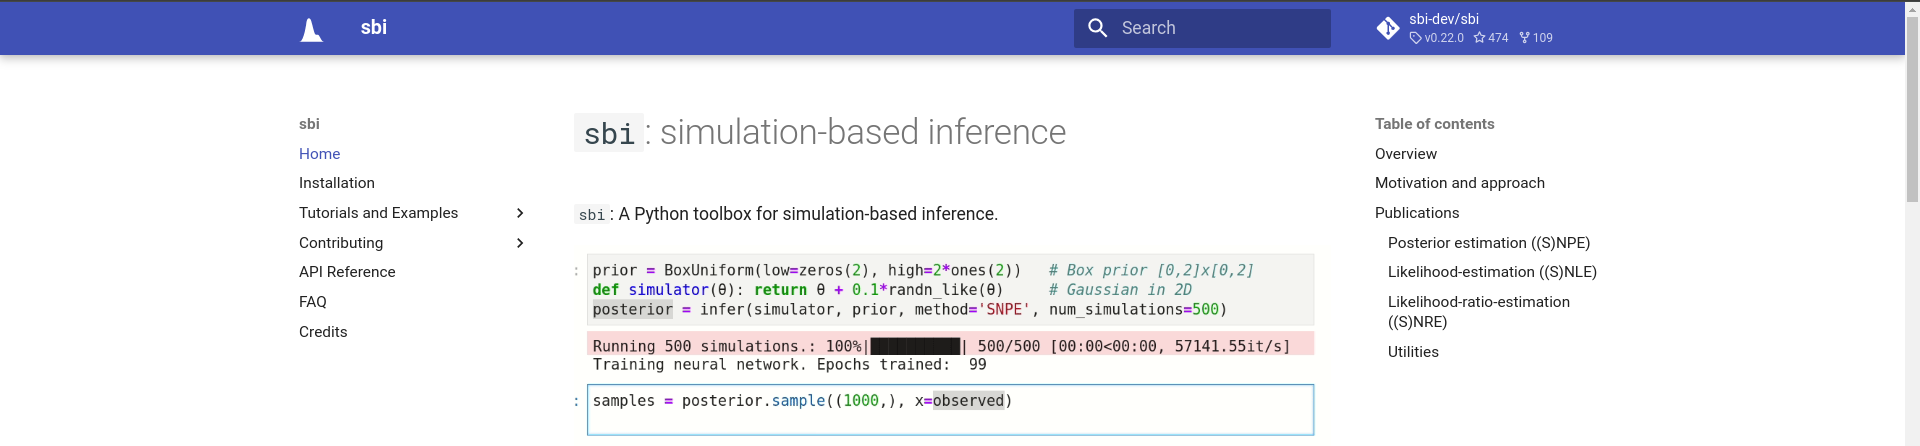
\includegraphics[width=\textwidth]{figures/sbi_screenshot}
        \href{https://github.com/sbi-dev}{github.com/sbi-dev}
        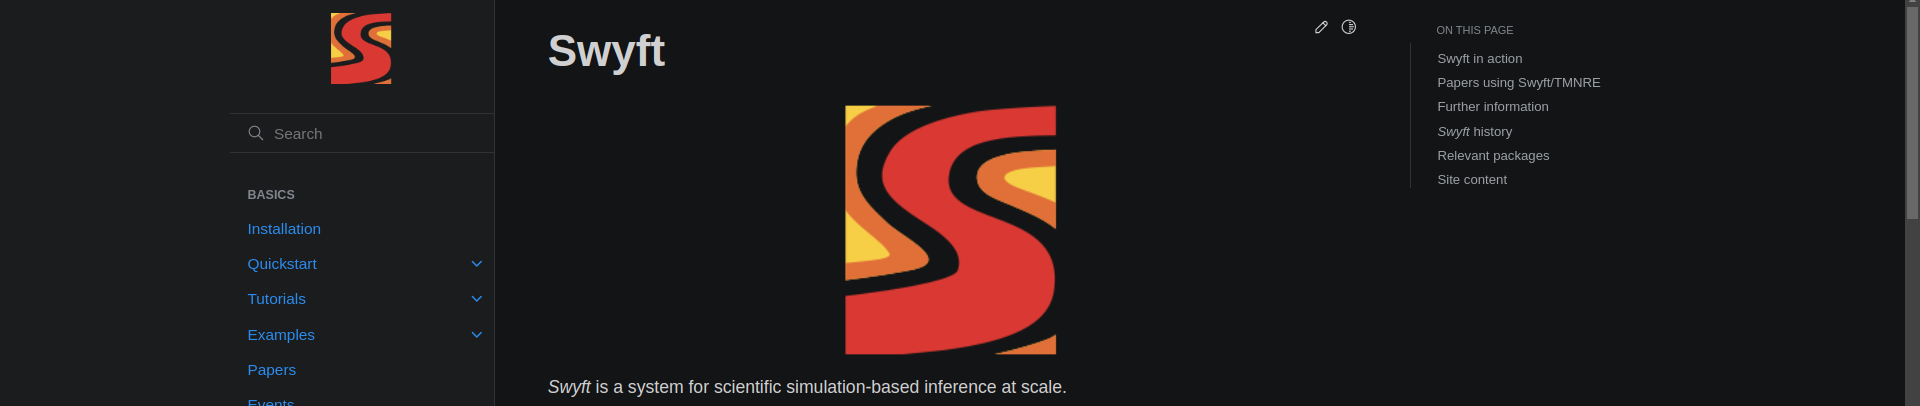
\includegraphics[width=\textwidth]{figures/swyft_screenshot}
        \href{https://github.com/undark-lab/swyft}{github.com/undark-lab/swyft}
        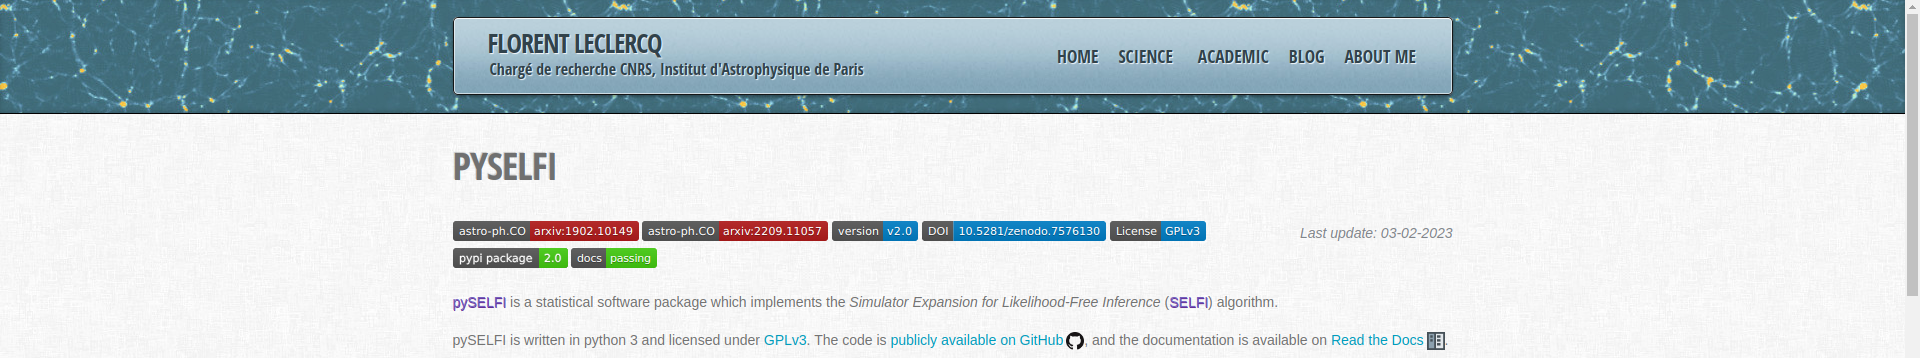
\includegraphics[width=\textwidth]{figures/selfi_screenshot}
        \href{https://github.com/florent-leclercq/pyselfi}{github.com/florent-leclercq/pyselfi}
        
\includegraphics[width=\textwidth]{figures/delfi_screenshot}
        \href{https://github.com/justinalsing/pydelfi}{github.com/justinalsing/pydelfi}
    \end{columns}
\end{frame}

\begin{frame}
    \frametitle{SBI in astrophysics}
    \begin{columns}
        \column{0.4\textwidth}
        \begin{itemize}
            \item 2024 has been the year it has started to be applied to real data.
            \item Mostly for weak lensing
            \item However: SBI requires mock data generation code
            \item Most data analysis codes were built before the generative paradigm.
            \item It's still a lot of work to upgrade cosmological likelihoods  to be able to do this (e.g.\ \texttt{plik} \& \texttt{camspec}).
        \end{itemize}
        \column{0.3\textwidth}
        
\includegraphics[width=\textwidth]{figures/sbi_papers/clusters.pdf}
        \vspace{10pt}\\
        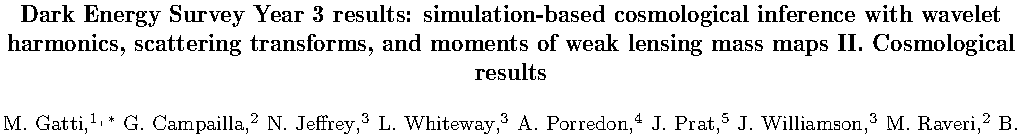
\includegraphics[width=\textwidth]{figures/sbi_papers/des.pdf}
        \vspace{10pt}\\
        
\includegraphics[width=\textwidth]{figures/sbi_papers/gw.pdf}
        \vspace{10pt}\\
        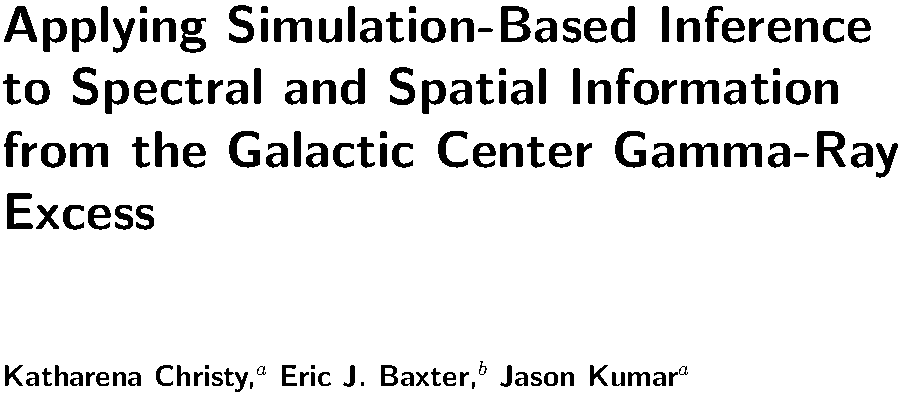
\includegraphics[width=\textwidth]{figures/sbi_papers/center.pdf}
        \column{0.3\textwidth}
        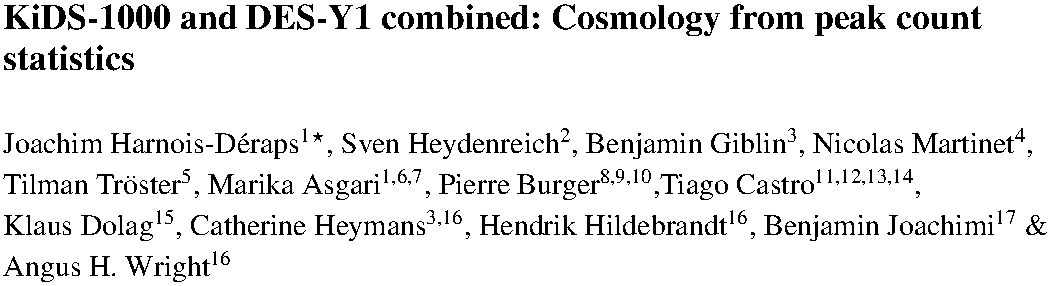
\includegraphics[width=\textwidth]{figures/sbi_papers/kidsdes.pdf}
        \vspace{10pt}\\
        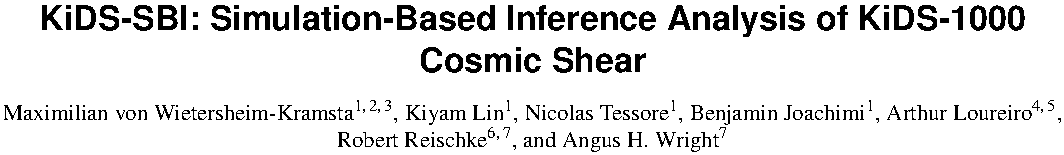
\includegraphics[width=\textwidth]{figures/sbi_papers/kids.pdf}
        \vspace{10pt}\\
        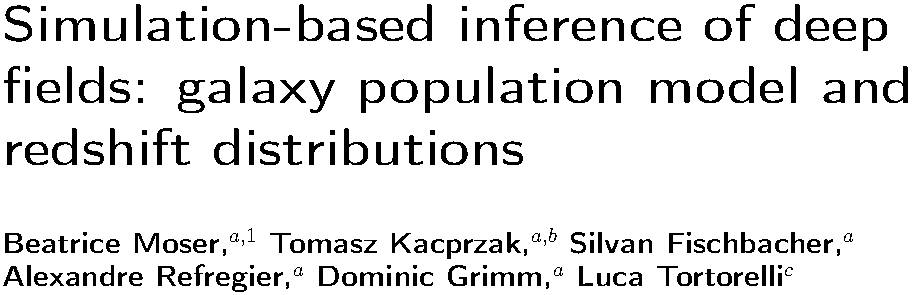
\includegraphics[width=\textwidth]{figures/sbi_papers/population.pdf}
        \vspace{10pt}\\
        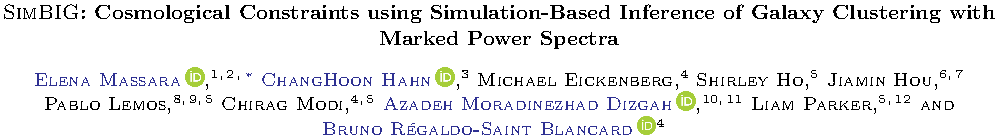
\includegraphics[width=\textwidth]{figures/sbi_papers/simbig.pdf}
    \end{columns}
\end{frame}

\subsection{Practice: NRE vs NDE}
\begin{frame}
    \frametitle{Neural Ratio Estimation}
    \begin{columns}
        \column{0.5\textwidth}
        \begin{itemize}
            \item SBI flavours: {\small \hfill\tthref{github.com/sbi-dev/sbi}}
                {\small
                    \begin{description}
                        \item[NPE] Neural posterior estimation
                        \item[NLE] Neural likelihood estimation
                        \item[NJE] Neural joint estimation
                        \item[NRE] Neural ratio estimation
                    \end{description}
                }
            \item NRE recap:
                \begin{enumerate}
                    \item Generate joint samples $(\theta,D)\sim\C[4]{\mathcal{J}}$
                        \label{step:joint}
                        \begin{itemize}
                            \item \textit{straightforward if you have a simulator:\\ $\theta\sim\C[1]{\pi(\cdot)}$, $D\sim\C[2]{\mathcal{L}(\cdot|\theta)}$}
                        \end{itemize}
                    \item Generate separated samples $\theta\sim\C[1]{\pi}$, $D\sim\C[3]{\mathcal{Z}}$\label{step:sep}
                        \begin{itemize}
                            \item \textit{aside: can shortcut step~\ref{step:sep} by scrambling the $(\theta,D)$ pairings from step~\ref{step:joint}}
                        \end{itemize}
                    \item Train probabilistic classifier $p$ to distinguish whether $(\theta,D)$ came from $\C[4]{\mathcal{J}}$ or $\C[1]{\pi}\times\C[3]{\mathcal{Z}}$.
                    \item $\frac{p}{1-p} = \C[5]{r} = \frac{P(\theta,D)}{P(\theta)P(D)} 
                        =
                        \frac{\C[4]{\mathcal{J}}}{\C[1]{\pi}\times\C[3]{\mathcal{Z}}} = \frac{\C[2]{\mathcal{L}}}{\C[3]{\mathcal{Z}}} = \frac{\C[0]{\mathcal{P}}}{\C[1]{\pi}}$.
                    \item Use ratio $\C[5]{r}$ for parameter estimation $\C[0]{\mathcal{P}} = \C[5]{r}\C[1]\times {\pi}$
                \end{enumerate}
        \end{itemize}
        \column{0.5\textwidth}
        \only<1|handout:0>{
            \begin{tikzpicture}[node distance=1cm, every neuron/.style={circle, draw, minimum size=1cm},]
                \node[every neuron/.try] (j2)  {};
                \node[every neuron/.try, above left = 0cm and 0.5cm of j2] (theta) { $\theta$};
                \node[every neuron/.try, below left = 0cm and 0.5cm of j2] (D) { $D$};
                \node[every neuron/.try, above = 0.5cm of j2] (j1) {};
                \node[every neuron/.try, below = 0.5cm of j2] (j3) {};
                \node[every neuron/.try, above right = 0cm and 0.5cm of j2] (h1) {};
                \node[every neuron/.try, below right = 0cm and 0.5cm of j2] (h2) {};
                \node[every neuron/.try, right = 1.3cm of j2] (p) { $p$};
                \node[every neuron/.try, right = 0.5cm of p] (logr) { $\C[5]{r}$};
                \draw[-] (theta) -- (j1);
                \draw[-] (D) -- (j1);
                \draw[-] (theta) -- (j2);
                \draw[-] (D) -- (j2);
                \draw[-] (theta) -- (j3);
                \draw[-] (D) -- (j3);
                \draw[-] (j1) -- (h1);
                \draw[-] (j1) -- (h2);
                \draw[-] (j2) -- (h1);
                \draw[-] (j2) -- (h2);
                \draw[-] (j3) -- (h1);
                \draw[-] (j3) -- (h2);
                \draw[-] (h1) -- (p);
                \draw[-] (h2) -- (p);
                \draw[-] (p) -- (logr);
                \node[below =0.5cm of logr] {\includegraphics[page=22, width=0.5\textwidth]{figures/sbi_parameter_estimation.pdf}};
            \end{tikzpicture}
        }
        \only<2>{
            \begin{exampleblock}{Bayesian proof}
                \begin{itemize}
                    \item Let $M_{\C[4]{\mathcal{J}}}$: $(\theta,D)\sim\C[4]{\mathcal{J}}$, $M_{\C[1]{\pi}\C[3]{\mathcal{Z}}}$: $(\theta,D)\sim\C[1]{\pi}\times\C[3]{\mathcal{Z}}$
                    \item Classifier gives
                        ${p(\theta,D) = P(M_{\C[4]{\mathcal{J}}}|\theta,D) = 1- P(M_{\C[1]{\pi}\C[3]{\mathcal{Z}}}|\theta,D)}$
                    \item Bayes theorem then shows
                        ${\frac{p}{1-p}=\frac{P(M_{\C[4]{\mathcal{J}}}|\theta,D)}{P(M_{\C[1]{\pi}\C[3]{\mathcal{Z}}}|\theta,D)} = \frac{P(\theta,D|M_{\C[4]{\mathcal{J}}})P(M_{\C[4]{\mathcal{J}}})}{P(\theta,D|M_{\C[1]{\pi}\C[3]{\mathcal{Z}}})P(M_{\C[1]{\pi}\C[3]{\mathcal{Z}}})} = 
                        \frac{\C[4]{\mathcal{J}}}{\C[1]{\pi}\C[3]{\mathcal{Z}}}}$, \\
                        where we have assumed 
                        \begin{itemize}
                            \item $P(M_{\C[4]{\mathcal{J}}}) = P(M_{\C[1]{\pi}\C[3]{\mathcal{Z}}})$,
                        \end{itemize}
                        and by definition
                        \begin{itemize}
                            \item $\C[4]{\mathcal{J}(\theta,D)} = P(\theta,D|M_{\C[4]{\mathcal{J}}})$
                            \item $\C[1]{\pi(\theta)}\C[3]{\mathcal{Z}(D)} = P(\theta,D|M_{\C[1]{\pi}\C[3]{\mathcal{Z}}})$.
                        \end{itemize}
                \end{itemize}
            \end{exampleblock}
        }
        \only<3|handout:0>{
            \begin{block}{Why I like NRE}
                \begin{itemize}
                    \item The link between classification and inference is profound.
                    \item Density estimation is hard -- Dimensionless $r$ divides out the hard-to-calculate parts.
                \end{itemize}
            \end{block}
            \begin{block}{Why I don't like NRE}
                \begin{itemize}
                    \item Practical implementations require marginalisation~\arxiv{2107.01214}, or autoregression~\arxiv{2308.08597}.
                    \item Model comparison and parameter estimation are separate~\arxiv{2305.11241}.
                \end{itemize}
            \end{block}
        }
    \end{columns}
\end{frame}

\section{GPU-accelerated inference}
\begin{frame}
    \frametitle{}
\end{frame}

\subsection{Accelerating with \texttt{jax}}
\begin{frame}[fragile]
    \frametitle{Jax-based nested samplers}
    \student{david_yallup}{David Yallup}{PDRA}
    \begin{itemize}
        \item \textbf{very} recent work over the past month
        \item Have implemented a nested slice sampler in \texttt{blackjax}~[\textcolor{C0}{\texttt{\href{https://github.com/blackjax-devs/blackjax/pull/755}{\#755}}}]
\begin{lstlisting}[language=Python]
pip install git+https://github.com/handley-lab/blackjax@nested_sampling
import blackjax.ns.adaptive\end{lstlisting}
        \item parallelised over \texttt{vmap}ped likelihood \& prior evaluations
        \item Plugs into \texttt{jim}~\arxiv{kazewong/jim} and \texttt{ripple}~\arxiv{2302.05329}
        \item interested in finding use-cases for such a sampler this week
        \item Also interested in understanding current limitations/strengths of $\texttt{jax}$/GPU GW programming
    \end{itemize}
\end{frame}


\begin{frame}
    \frametitle{\ldots}
\hfill \textit{Frontiers of simulation based inference}~\arxiv{1911.01429}
    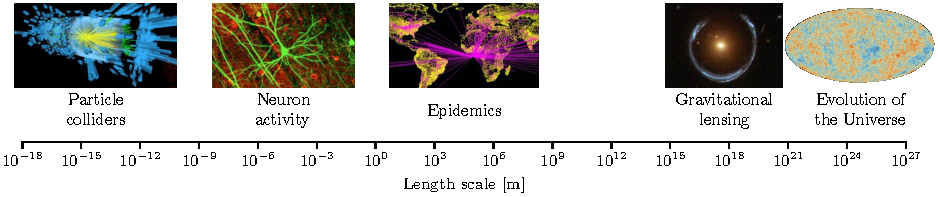
\includegraphics[width=\textwidth]{figures/sbi_range.pdf}
\end{frame}

\begin{frame}
    \frametitle{Conclusions}
    \framesubtitle{\tthref{github.com/handley-lab/group}}
    \tikz[overlay,remember picture]
        \node[anchor=north east] (A) at ($(current page.north east)+(0,0)$) {
        
\includegraphics[width=0.09\textheight]{people/adam_ormondroyd.jpg}%
        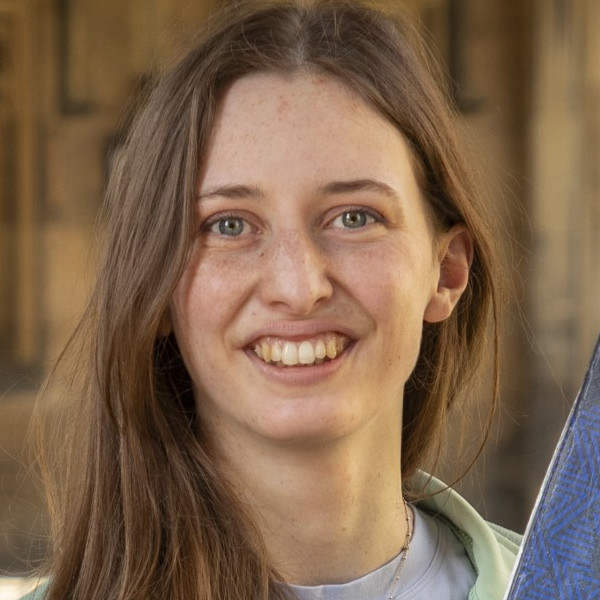
\includegraphics[width=0.09\textheight]{people/charlotte_priestley.jpg}%
        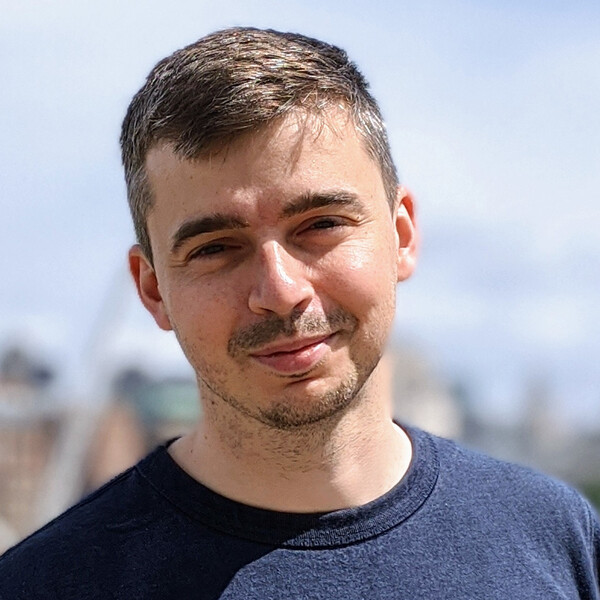
\includegraphics[width=0.09\textheight]{people/david_yallup.jpg}%
        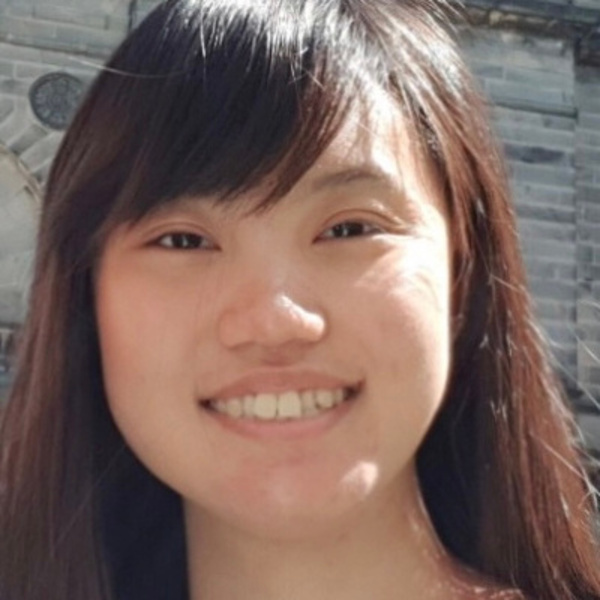
\includegraphics[width=0.09\textheight]{people/dily_ong.jpg}%
        
\includegraphics[width=0.09\textheight]{people/harry_bevins.jpg}%
        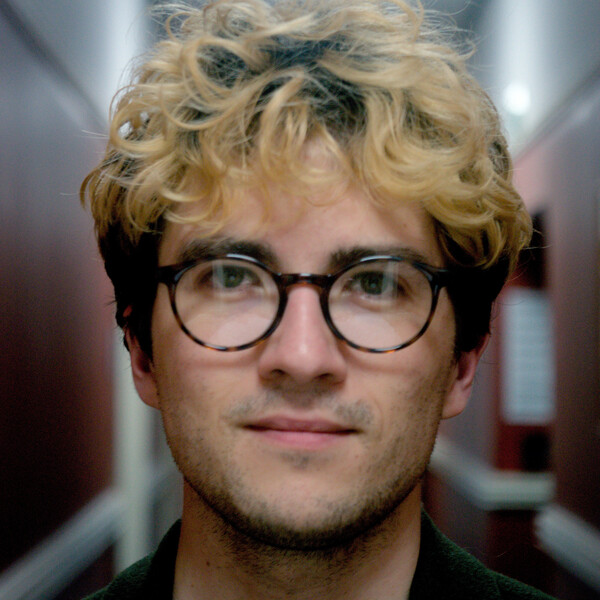
\includegraphics[width=0.09\textheight]{people/harvey_williams.jpg}%
        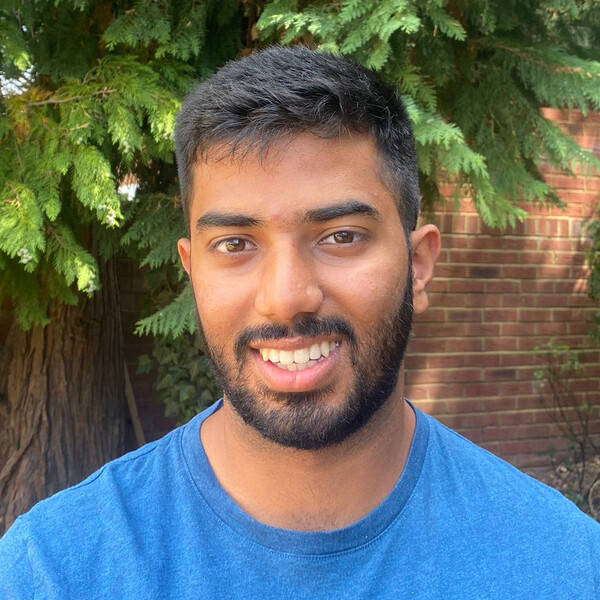
\includegraphics[width=0.09\textheight]{people/krish_nanavati.jpg}%
        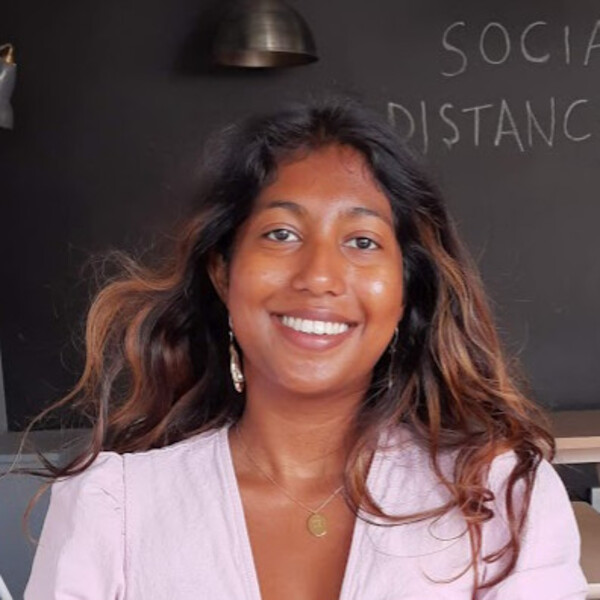
\includegraphics[width=0.09\textheight]{people/metha_prathaban.jpg}%
        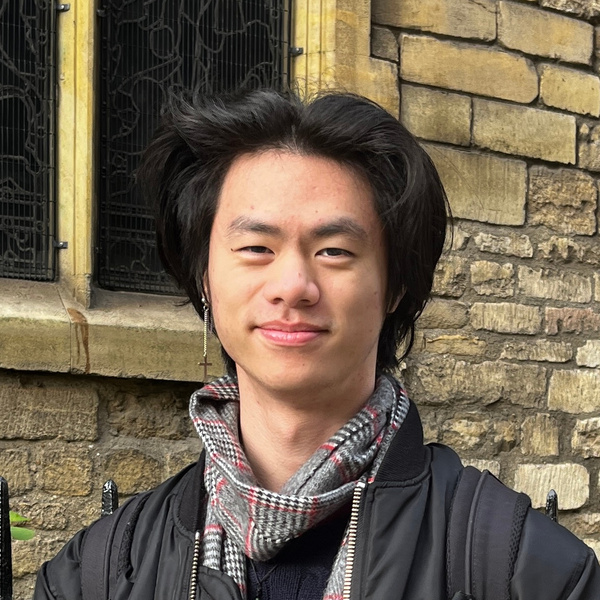
\includegraphics[width=0.09\textheight]{people/ming_yang.jpg}%
        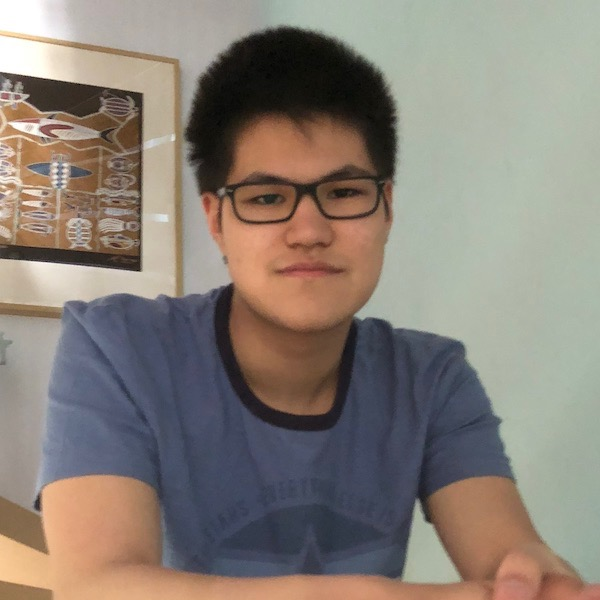
\includegraphics[width=0.09\textheight]{people/namu_kroupa.jpg}%
        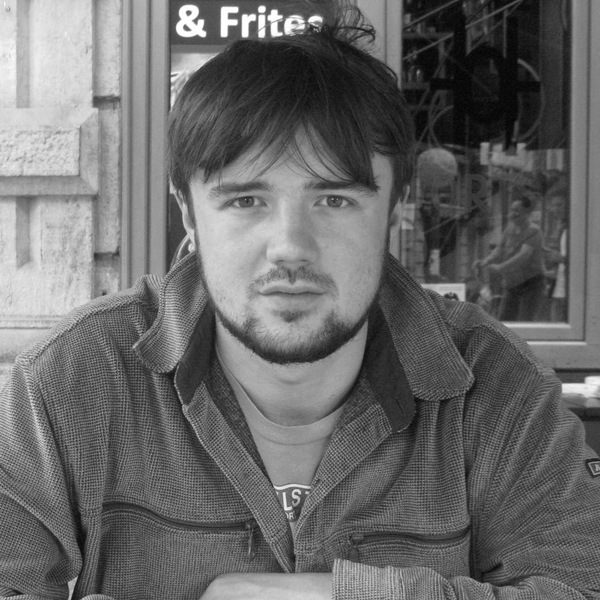
\includegraphics[width=0.09\textheight]{people/sam_leeney.jpg}%
        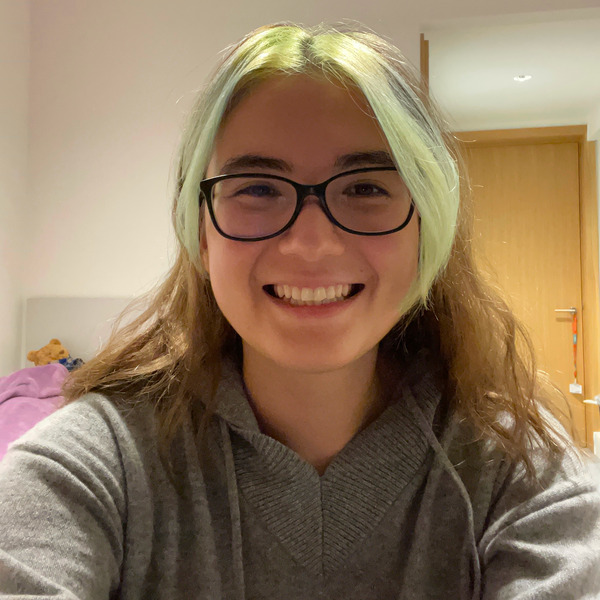
\includegraphics[width=0.09\textheight]{people/sinah_legner.jpg}%
        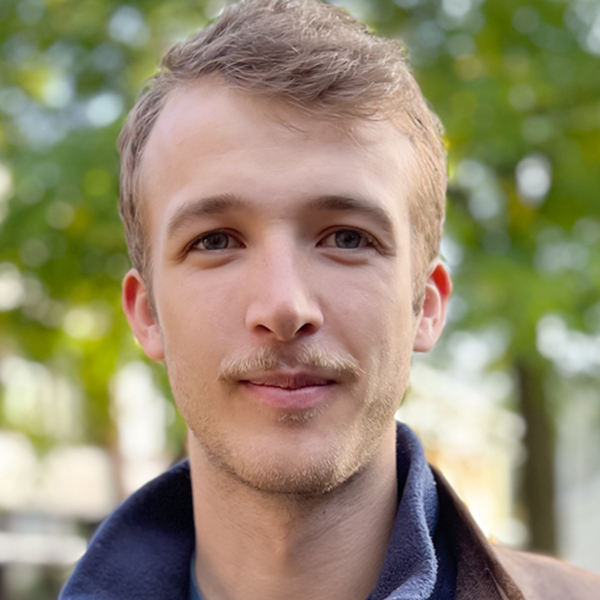
\includegraphics[width=0.09\textheight]{people/toby_lovick.jpg}%
        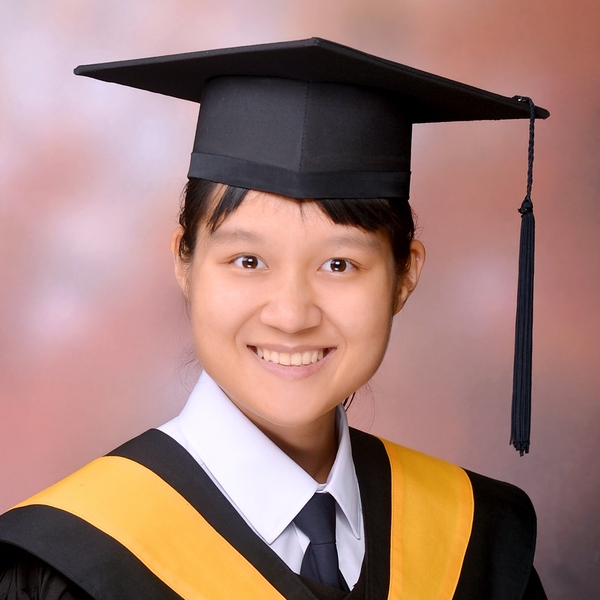
\includegraphics[width=0.09\textheight]{people/wei-ning_deng.jpg}%
        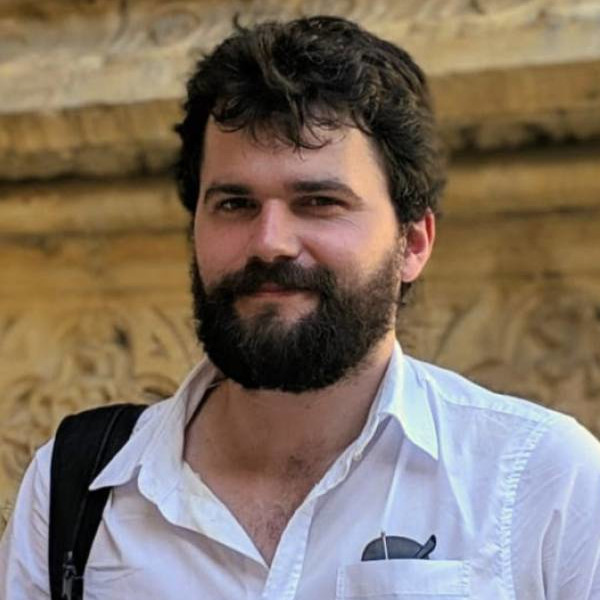
\includegraphics[width=0.09\textheight]{people/will_handley.jpg}%
        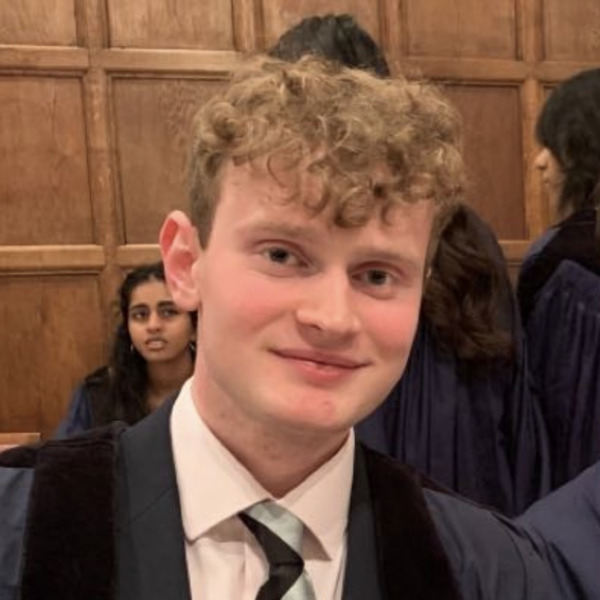
\includegraphics[width=0.09\textheight]{people/will_templeton.jpg}%
    };
\end{frame}

\end{document}
